\section{Theorie}
\label{sec:Theorie}
\subsection{Grundlagen}
Ultraschallwellen sind Schallwellen im Frequenzbereich von $\SI{20}{\kilo\hertz}$ bis
$\SI{1}{\giga\hertz}$ mit denen die Struktur von Materialien untersucht werden kann.
Schallwellen sind longitudinale Wellen der Form
\begin{equation}
	p(x,t) = p_0 + v_0 Z \cos(\omega t - kx) \mathrm{,}
\end{equation}
wobei $Z$ als akustische Impedanz oder Schallkennwiderstand bezeichnet wird.
Schallwellen können -- wie elektromagnetische Wellen -- reflektiert und gebrochen werden.
Da sie sich aber aufgrund von Druckschwankungen im Raum fortbewegen, ist die
Schallgeschwindigkeit $c$ materialabhängig. Bei Flüssigkeiten zum Beispiel hängt die
Schallgeschwindigkeit von der Kompressibilität $\kappa$ und der Dichte $\rho$ ab;
\begin{equation}
	c_{\mathrm{Fl}} = \sqrt{\frac{1}{\kappa\rho}} \, \mathrm{.}
\end{equation}
Die Schallgeschwindigkeit in Festkörpern ergibt sich durch
\begin{equation}
	c_{\mathrm{Fe}} = \sqrt{\frac{E}{\rho}} \, \mathrm{,}
\end{equation}
mit dem Elastizitätsmodul $E$.
Damit lässt sich die akustische Impedanz
\begin{equation}
	Z=c \rho
\end{equation}
bestimmen.
Des Weiteren wird Schall von dem Material absorbiert, sodass die Schallamplitude exponentiell
mit dem Ort $x$ abfällt;
\begin{equation}
	\label{eqn:dampf}
	I(x) = I_0 \, \symup{e}^{-\alpha x} \mathrm{.}
\end{equation}
Die Absorptionsstärke wird vom materialabhängigen Absorptionskoeffzienten $\alpha$ festgelegt.
Luft beispielsweise absorbiert Schall sehr stark, sodass in der Praxis ein Kontaktmittel an der
Grenzfläche von dem untersuchten Material aufgetragen wird.
Wenn Schall auf eine Grenzfläche trifft, wird ein Teil reflektiert -- der Anteil wird durch den
Reflexionskoeffizienten
\begin{wrapfigure}{R}{5cm}
	\centering
	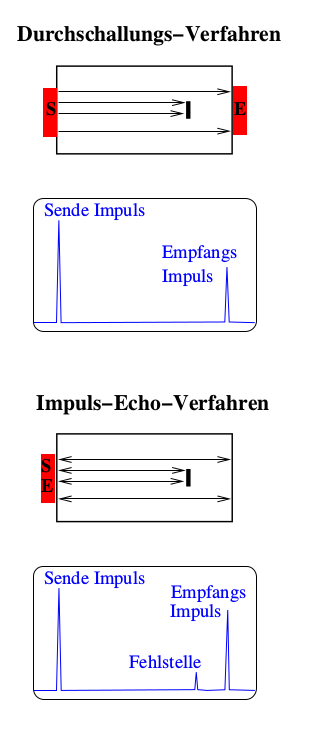
\includegraphics[width=0.25\textwidth]{Bilder/Messverfahren.png}
	\caption{Prinzipielle Darstellung der Messverfahren. \cite{Anleitung}}
	\label{fig:echo}
\end{wrapfigure}
\begin{equation}
	R =(\frac{Z_1-Z_2}{Z_1+Z_2})^2
\end{equation}
bestimmt -- und ein Teil transmittiert (Anteil ergibt sich aus $T=1-R$).

Ultraschall kann beispielsweise mit dem piezo-elektrischen Effekt erzeugt werden.
Durch ein elektrisches Wechselfeld kann ein piezo-elektrischer Kristall -- z.B. Quarze -- zu
Schwingungen angeregt werden. Wird der Kristall mit
